
\section{Test Cases (Old)}
\label{sec:test_cases_old}

For these cases, unless otherwise specified, we use a regularization given by
$\alpha=1.0$. 
\todo{This is old and makes reference to the rigid approximation. I think makes sense to instead use true compliance and it'd simplify the analysis.}

\subsection{Conveyor Belt}
\label{sec:conveyor_belt}

In this case a box of mass $m=1~\text{kg}$ that is only allowed to move in the
vertical direction is placed on top of a conveyor belt moving horizontally in
the $-x$ direction with a specified velocity $u_0=-0.1~\text{m}/\text{s}$, Fig.
\ref{fig:conveyor_belt}. The coefficient of friction is $\mu=0.5$.

\begin{figure}[!h]
	\centering
	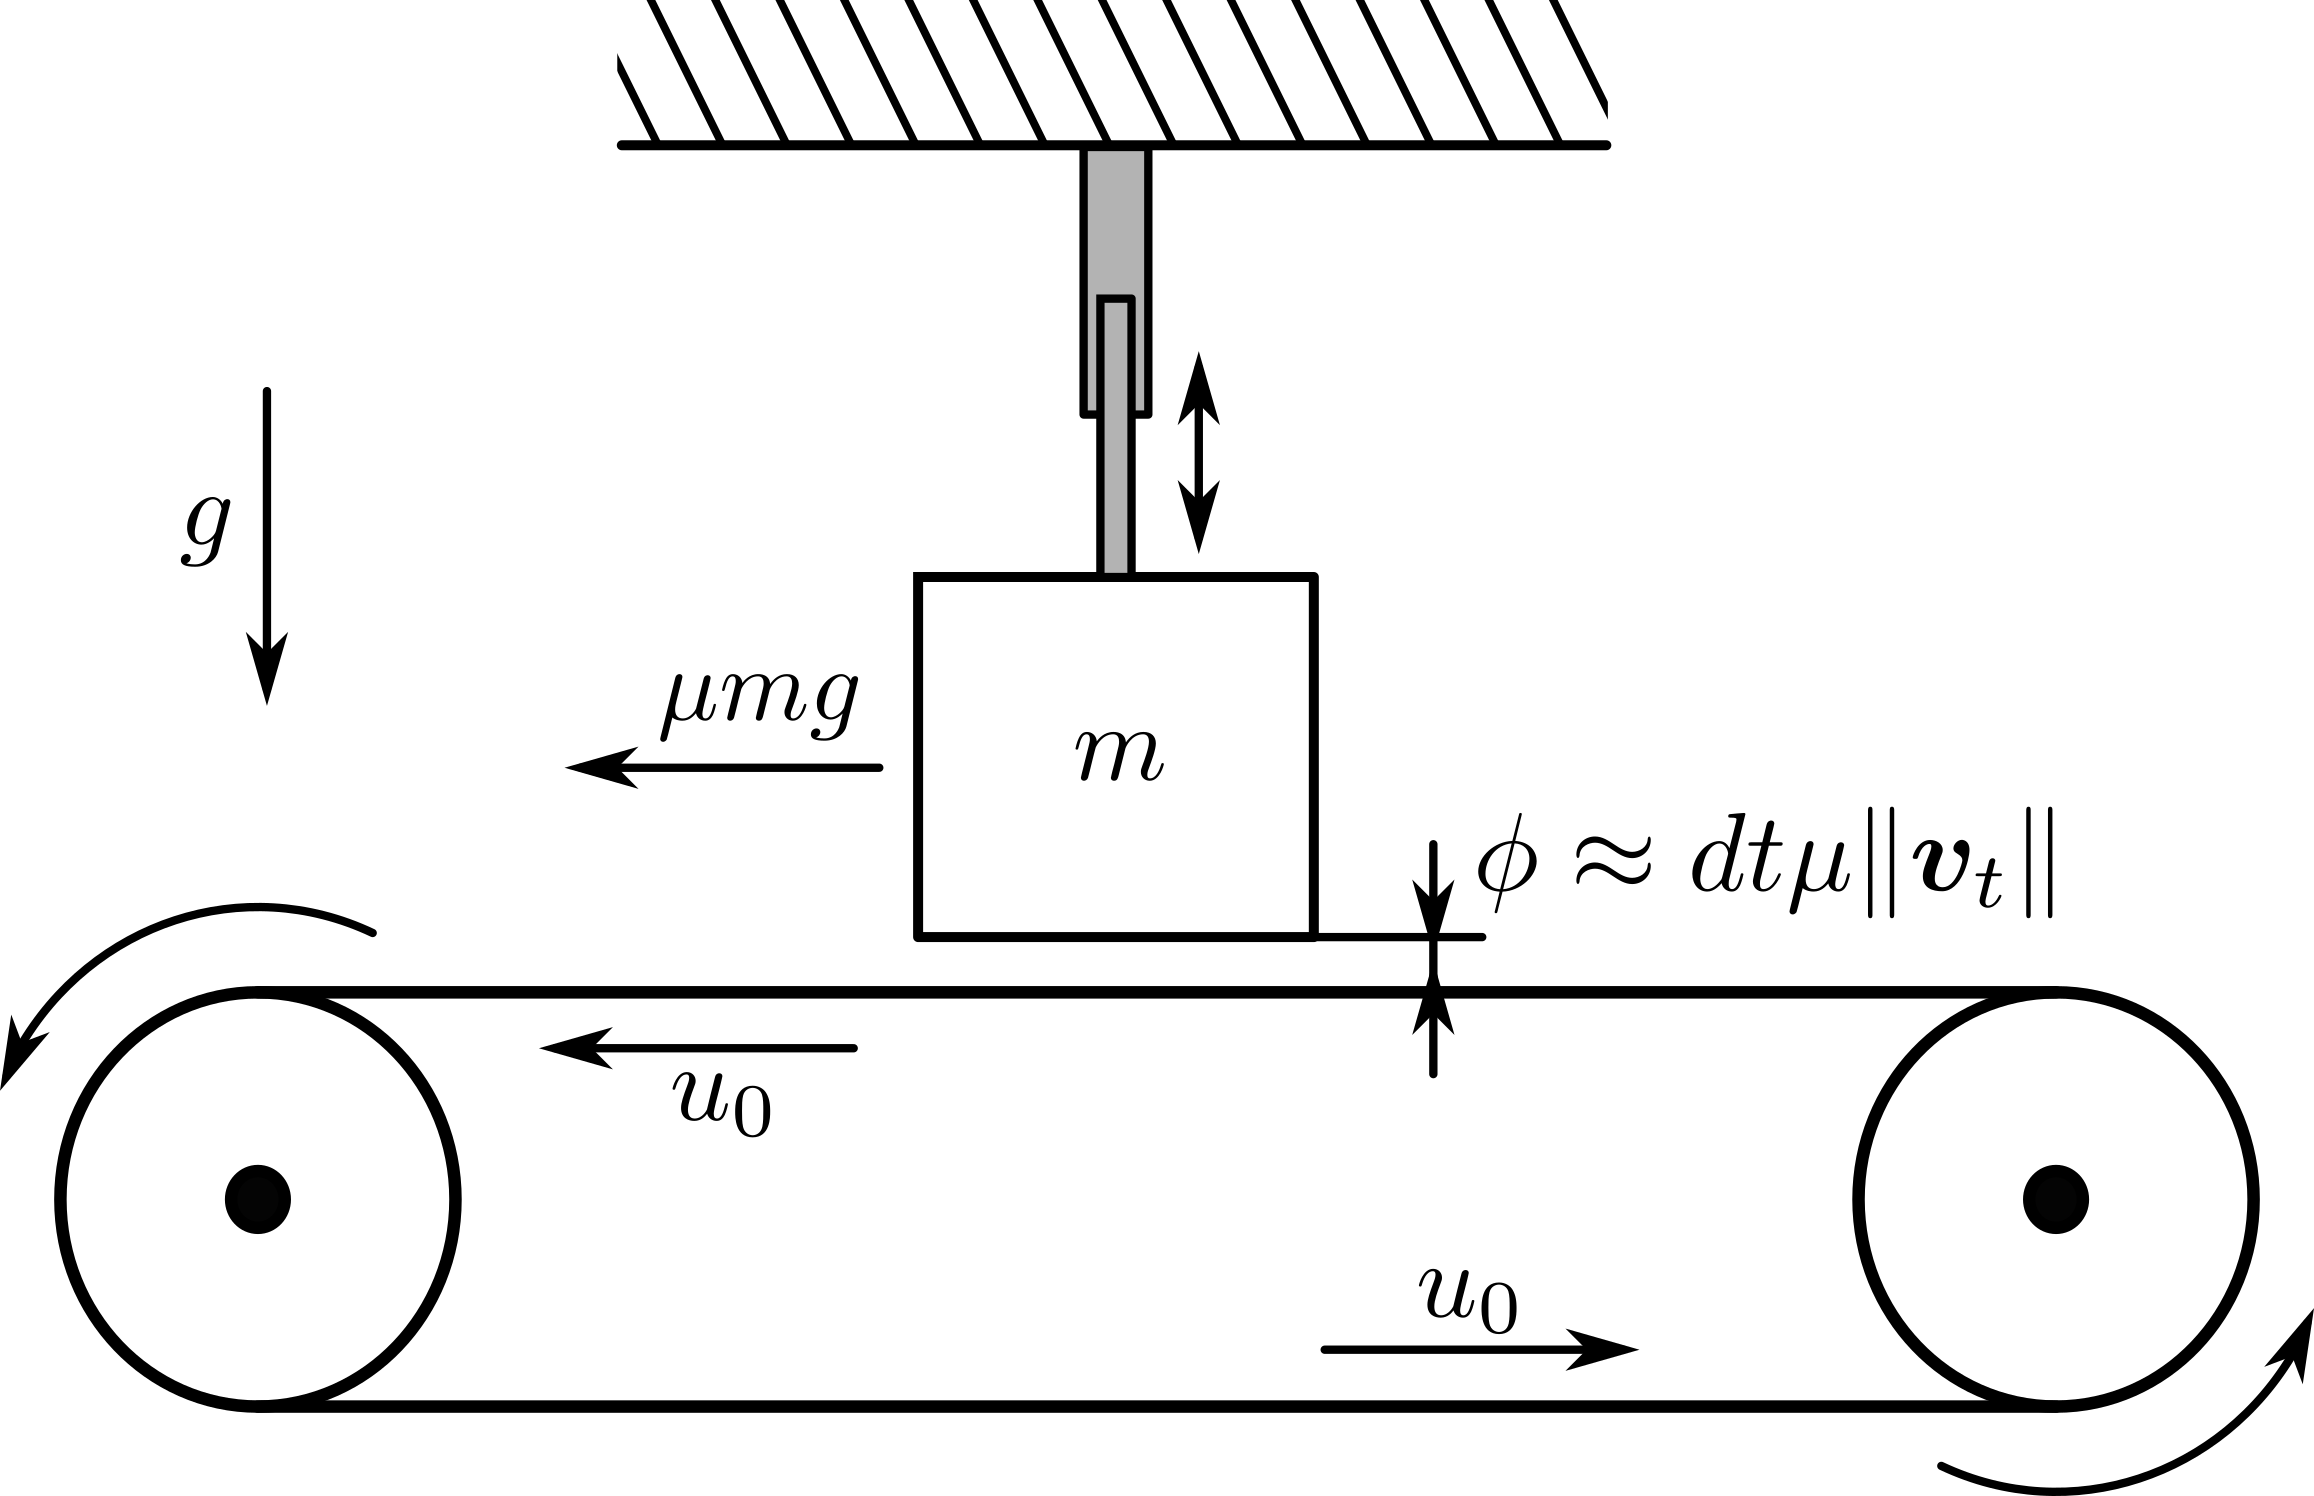
\includegraphics[width=0.4\columnwidth]{figures/conveyor_belt/conveyor_belt.png}
	\caption{\label{fig:conveyor_belt} 
	Schematic of the conveyor belt case highlighting the \textit{gliding
	artifact} during sliding.}
\end{figure}

Given the regularization used in this formulation, a given amount of compliance
given by $R_n$ is expected and therefore the box will initially undergo a
vertical motion until the \textit{compliant} normal force balances the weight of
the box. We will see however that due to the convex regularization the vertical
motion is not only given by the normal compliance but also by the sliding
velocity at contact.

We run this simulation using time steps in a geometric sequence with a common
ration $\sqrt{10}$. Starting with the smallest value of $dt = 10^{-4}~\text{s}$
to the larger value of $dt = 10^{-2}~\text{s}$.

\subsubsection{Steady state solution}
In the steady state the normal impulse $\gamma_n$ will balance the weight of box
$P=m\,g$, i.e. $\gamma_n=dt\,m\,g$. Also the normal velocity will be zero and
therefore we can find out the steady state value of the signed distance $\phi$,
or similarly the value of the stabilization velocity $b=\phi/dt$, from the
analytical inverse dynamics Eq. \ref{eq:inverse_dynamics_velocity} as
\begin{eqnarray}
	b=\frac{\phi}{dt}=\mu\Vert\vf{v}_t\Vert-(1+\tilde\mu^2)R_n\gamma_n
\end{eqnarray}

For this problem we have that $\mf{J}_c=[0, 0, 1]^T$ and $\mf{M}=m$ and thus the
Delassus operator is
\begin{equation}
	\mf{W} = \begin{bmatrix}
		0 & 0 & 0\\
		0 & 0 & 0\\
		0 & 0 & 1/m\\
		\end{bmatrix}
\end{equation}
and therefore $g_i=(3m)^{-1}$.

Using the fact that $R_n=\varepsilon_n\,g_i = \frac{\alpha^2}{4\pi^2}g_i$, and
that $\gamma_n=dt\,m\,g$ we can write the final expression for $b$ as
\begin{eqnarray}
	b=\frac{\phi}{dt}=\mu\Vert\vf{v}_t\Vert-(1+\tilde\mu^2)\frac{\alpha^2}{12\pi^2}g\,dt
	\label{eq:conveyor_belt_analytic}
\end{eqnarray}

In our regularization, $\alpha$ controls the amount of \textit{compliance}. In
the limit $\alpha\rightarrow 0$ we approach the rigid limit. Equation
\ref{eq:conveyor_belt_analytic} shows us that in this limit the signed distance
approaches the \textit{positive} value $\phi = dt\mu\Vert\vf{v}_t\Vert$. This is
consistent with previous work using Anitescu's formulation which does not
introduce regularization, see \cite{bib:anitescu2006, bib:mazhar2014}.

\subsubsection{Initial conditions}
If we replace values for $\alpha=1.0$, $g=10~\text{m}/\text{s}^2$ and a range of
time steps, we find out that the effect of normal compliance is much smaller
than the rigid limit value $\phi = dt\mu\Vert\vf{v}_t\Vert$ and thus $\phi$ in
this problem is positive for relevant parameter values. This means that if we
use an initial condition of $\phi=0$ (rigid contact), the formulation will
generate a very large impulse in order to violently push the box away from the
moving belt. Therefore we prefer to initialize the vertical position of the box
such that $\phi = dt\mu|u_0|$ to avoid this impulsive behavior.

\subsubsection{Simulation results}

Starting with the box at $z=dt\mu|u_0|$ and $\dot{z}=0$ we simulate forward the
dynamics of the box for $0.15$ seconds, long enough to reach a steady state at
which the normal compliance result from regularization balances the weight of
the box.

Figure \ref{fig:phi_over_h_Rt_comparison} plots the value of $b=\phi/dt$ for a
range of time steps and two different values of $\sigma_t$ ($R_t=\sigma_tR_n$).
As predicted by Eq. (\ref{eq:conveyor_belt_analytic}), in the limit
$dt\rightarrow 0$ we have that
$b=\phi/dt=\mu\Vert\vf{v}_t\Vert=0.05~\text{m}/\text{s}$. As the time step
increases, the effect of the numerical compliance introduced for regularization
becomes more evident and this value drops as the box sinks deeper into the
moving belt. The value of $R_t$ has a weaker though noticeable effect given the
term $(1+\tilde\mu^2)$ in Eq. (\ref{eq:conveyor_belt_analytic}).
%
\begin{figure}[!h]
	\centering
	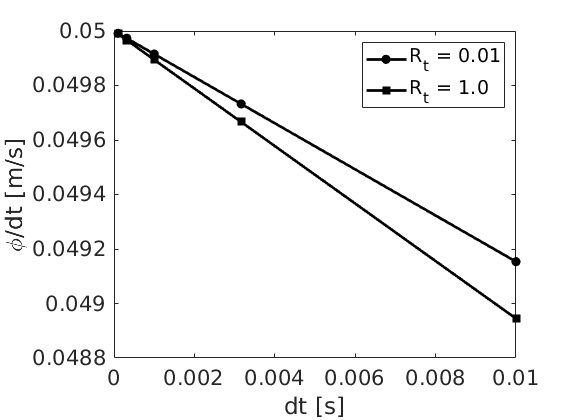
\includegraphics[width=0.5\textwidth]{figures/conveyor_belt/phi_over_h_Rt_comparison.png}
	\caption{\label{fig:phi_over_h_Rt_comparison} 
	Steady state value of the \textit{stabilization velocity} $b=\phi/dt$ as a
	function of the time step $dt$. As the time step approaches zero the scheme
	approximates to the \textit{rigid} solution at which
	$\phi/dt\rightarrow\mu\Vert\vf{v}_t\Vert$. The slope of this line is
	consistent with the analytical solution in Eq.
	(\ref{eq:conveyor_belt_analytic}) due to the numerical compliance introduced
	by the regularization terms. The slope increases with larger values of $R_t$
	as predicted by Eq. (\ref{eq:conveyor_belt_analytic}).}
\end{figure}

The dynamics of the initial transient is shown in Fig.
\ref{fig:normal_velocity}, which plots velocity a s function of time. It is
interesting to note that when both time and velocity are normalized by the step
size, solution results using different step sizes collapse into a single curve.
From Fig. \ref{fig:normal_velocity} we see that the initial transient lasts for
about four time steps, regardless of the step size. We also observe that the
normal velocity values are larger for larger time steps. This is consistent with
the results in Fig. \ref{fig:phi_over_h_Rt_comparison} since larger time steps
lead to larger compliance and larger values of $\phi$. 


\begin{figure}[!h]
	\centering
	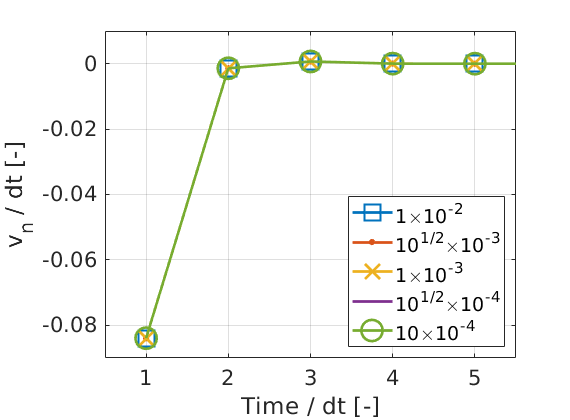
\includegraphics[width=0.5\textwidth]{figures/conveyor_belt/normal_velocity.png}
	\caption{\label{fig:normal_velocity} 
	Normal velocity as a function of time. Simulation results using different
	time steps collapse into a single curve when both velocity and time are
	normalized using the time step.}
\end{figure}

\subsection{Sliding box}
\label{sec:sliding_box}

In this case a box of mass $m=1~\text{kg}$ with given an initial horizontal
velocity $v=[1.0, 0.0, 0.0]~\text{m}/\text{s}$ slides on the ground with
friction coefficient $\mu=0.5$ until it stops, see Fig. \ref{fig:sliding_box}.
The case is run with two time steps, $dt=10^{-2}~\text{s}$ and
$dt=10^{-3}~\text{s}$.

\begin{figure}[!h]
	\centering
	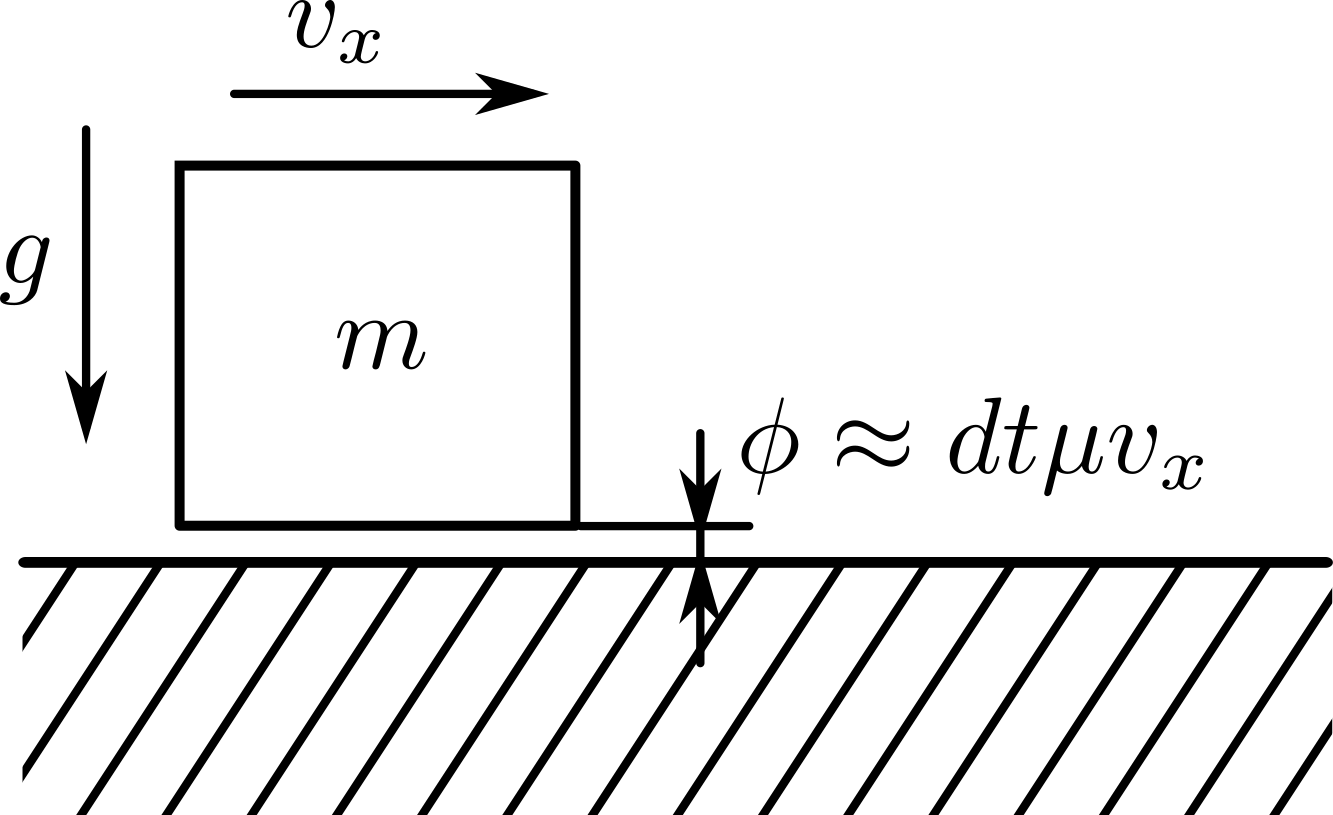
\includegraphics[width=0.3\columnwidth]{figures/sliding_box/sliding_box.png}
	\caption{\label{fig:sliding_box} 
	Schematic of the sliding box case highlighting the \textit{gliding artifact}
	during sliding.}
\end{figure}

\subsubsection{Inconsistent initial conditions}
The naive initial condition for this case is to set the box to be in imminent
contact with the ground, i.e. $z = 0$. We would think that the box would
slightly sink into the ground due to the numerical compliance introduced by
regularization, as we learned from Section \ref{sec:conveyor_belt}. However we
quickly find out from the Fig. (\ref{fig:sliding_box}) that this is not the
case. Nevertheless we do find that this is a consistent results previously
reported in \cite{bib:mazhar2014}. However the cause of this apparent artifact
of the formulation is not investigated further in \cite{bib:mazhar2014}.

The answer to why we obtain this solution becomes evident when looking at the
forces in Fig. (\ref{fig:sliding_box}). We find out that there is an initial
large impulse at the very first time step and forces go to zero immediately
after. The reason, is that this very large impulse pushed the box upwards into a
short free flight trajectory. This explains the vertical velocity profile in
Fig. (\ref{fig:sliding_box}) with the vertical velocity decreasing only due to
the acceleration of gravity. The question now is, why is it that in the very
first time step we obtain this very large impulse? the situation doesn't seem to
improve when reducing the time step. The answer lies in the previous case in
Section \ref{sec:conveyor_belt}. We learned that when a contact is sliding, the
contact distance will be slightly positive and approximately given by $z\approx
dt\mu\Vert\vf{v}_t\Vert$. Therefore, when we initialize the problem with $z=0$,
this effectively sets the problem with a constraint violation given by $z\approx
dt\mu\Vert\vf{v}_t\Vert$ and the solver must violently push the box out of this
configuration. This initial transient is so violent that sets the box on free
flight for almost $0.1$ seconds.

\subsubsection{Consistent initial conditions}
The solution is then to initialize the box with $z= dt\mu\Vert\vf{v}_t\Vert$.
The reader might argue that in general this is not possible. However, keep in
mind that this kind of problems is impulsive and not quite physical. The reason
is that in this problem the box is already in motion at $t=0$ while in the real
world we'd need to accelerate the box to that velocity in a finite time, giving
the formulation enough time to settle to a proper value of $z$ consistent with
the contact constraints. For the sake of understanding this effect however, we
set now the initial height of the box to $z= dt\mu\Vert\vf{v}_t\Vert$.

The new solution is shown in Fig. (\ref{fig:sliding_box_phi0}). Even though
there is a small transient at the beginning of the simulation due to the
numerical compliance introduced by the regularization, the solution is
significantly smoother and better approximates the real problem we want to
solve; the normal force $f_n=10~\text{N}$ quickly settles to balance the weight,
the horizontal forces settles to the sliding force $f_t=-\mu\,f_n=5~\text{N}$
and the horizontal velocity decelerates at constant rate to a full stop.

\subsubsection{Convex relaxation artifacts}

We essentially observe three different artifacts in Fig.
(\ref{fig:sliding_box_phi0}). The first one is the initial transient lasting
about $~4$ time steps. This is related to the numerical compliance introduced by
the regularization. As we learned from Fig. (\ref{fig:phi_over_h_Rt_comparison})
compliance leads to a signed distance value that is slightly smaller than
$dt\mu\Vert\vf{v}_t\Vert$. 

The second artifact is the small negative vertical velocity as the box is
sliding. This requires more analysis but we can explain it. As we learned, the
box will glide at a distance from the ground approximately equal to $z\approx
dt\mu\Vert\vf{v}_t\Vert$. However the box is decelerating at a constant rate due
to the Coulomb friction force, i.e. $\dot{v}_t\approx -\mu g$. Therefore we can
estimate the normal velocity as $v_n=\dot{z}\approx dt\mu \dot{v}_t=dt\mu^2g$.
This leads to the estimation $v_n\approx 2.5\times 10^{-2}~\text{m}/\text{s}$
when $dt=10^{-2}~\text{s}$ and $v_n\approx 2.5\times 10^{-3}~\text{m}/\text{s}$
when $dt=10^{-3}~\text{s}$, which is in perfect agreement with the results shown
in Fig. (\ref{fig:sliding_box_phi0}).

The final and third artifact is the small peak in the normal force, which is not
present in the true physical solution. Interestingly, this peak seems to have a
magnitude independent of the time step. A deeper analysis will also explain
this. When the box finally transitions to stiction, velocity drops to zero, as
we see in the figure. As we already saw, there is a non-zero normal velocity
$v_n$ as the box slides and this velocity goes to zero when the box enters into
stiction. Therefore there is a finite velocity change of magnitude $v_n$, an
impact, that leads to an impulse $\Delta\gamma_n\approx m\,v_n\approx
dt\mu^2m\,g$. The change in the normal force is then $\Delta
f_n=\Delta\gamma_n/dt\approx \mu^2m\,g \approx 2.5~\text{N}$, independent of the
time step. The peak in Fig. (\ref{fig:sliding_box_phi0}) is slightly below 2 N,
consistent with our estimation since careful inspection of the results show us
that velocity does not go to zero in a single step but rather it takes about two
steps and therefore the impulsive response has a wider support and smaller
magnitude.

\begin{figure}[!h]
	\centering
	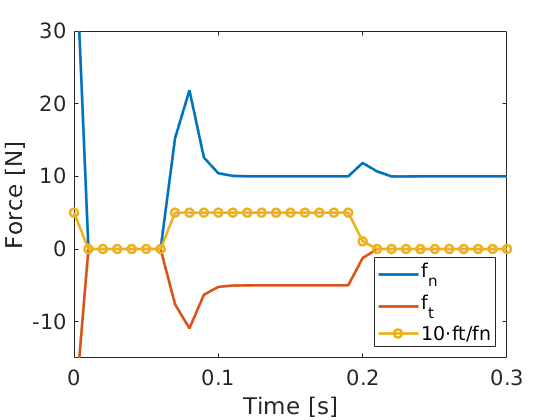
\includegraphics[width=0.45\columnwidth]{figures/sliding_box/forces_h1em2.png}
    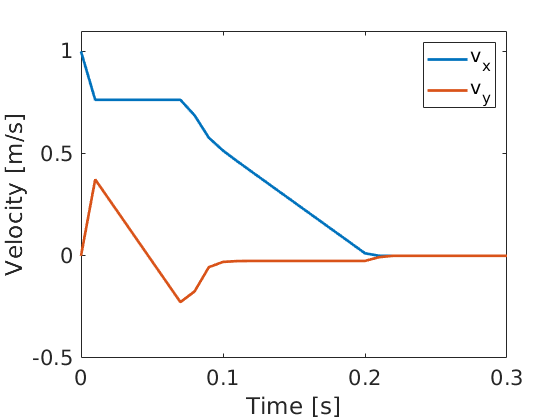
\includegraphics[width=0.45\columnwidth]{figures/sliding_box/velocities_h1em2.png}\\
    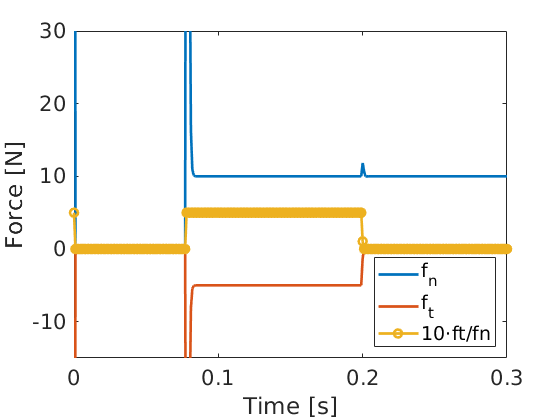
\includegraphics[width=0.45\columnwidth]{figures/sliding_box/forces_h1em3.png}
    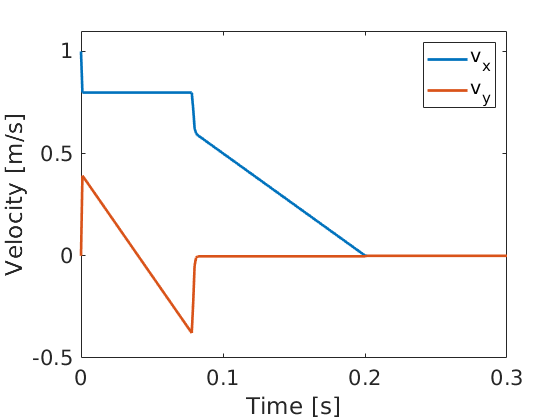
\includegraphics[width=0.45\columnwidth]{figures/sliding_box/velocities_h1em3.png}\\
	\caption{\label{fig:sliding_box} 
	Horizontal $u$ and vertical $v$ velocities (left) and contact forces (right)
	as a function of time. Osccillations during sliding are a consequence of the
	convex relaxation which introduces a dependence of the normal forces on the
	sliding velocity.}
\end{figure}

\begin{figure}[!h]
	\centering
	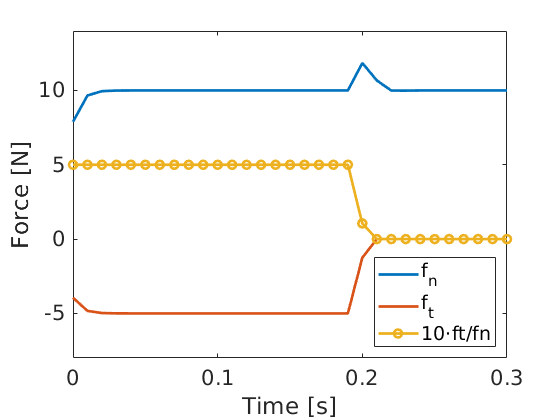
\includegraphics[width=0.45\columnwidth]{figures/sliding_box/forces_h1em2_phi0.png}
    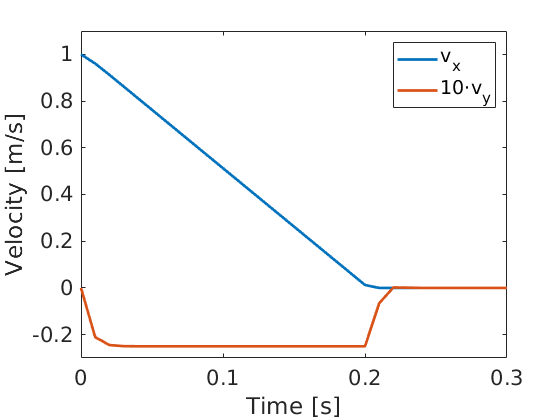
\includegraphics[width=0.45\columnwidth]{figures/sliding_box/velocities_h1em2_phi0.png}\\
    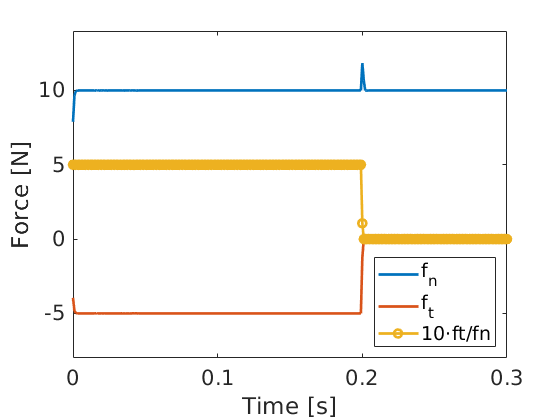
\includegraphics[width=0.45\columnwidth]{figures/sliding_box/forces_h1em3_phi0.png}
    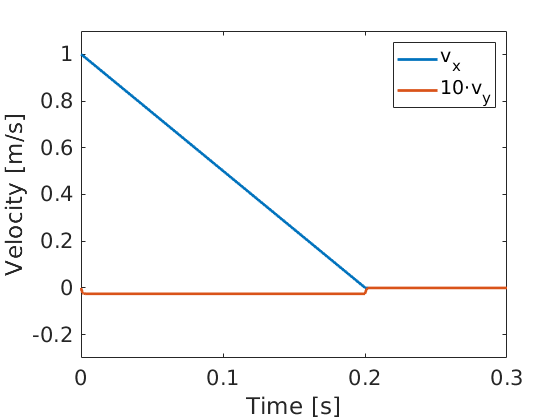
\includegraphics[width=0.45\columnwidth]{figures/sliding_box/velocities_h1em3_phi0.png}\\
	\caption{\label{fig:sliding_box_phi0} 
	Horizontal $u$ and vertical $v$ velocities (left) and contact forces (right)
	as a function of time. Osccillations during sliding are a consequence of the
	convex relaxation which introduces a dependence of the normal forces on the
	sliding velocity.}
\end{figure}

\subsection{Clutter}
\label{sec:clutter}

The purpose of this case is to evaluate the scalability of this method with
problem size. The setup consists of an open container of
$80~\text{cm}\times80~\text{cm}$ and $40~\text{cm}$ of height. Objects are
dropped into this container from four different piles of five objects each, as
shown in the upper left corner of Fig. \ref{fig:clutter}. Each pile consists of
an arbitrary assortment of spheres of radii $5~\text{cm}$ and boxes with sides
$10~\text{cm}$ in length. To emulate multi-contact, boxes are augmented with an
array of $3\times 3$ points on each face, shown as red spheres in Fig.
\ref{fig:clutter}.

Figure \ref{fig:clutter} shows snapshots of the solution computed with
$dt=10^{-2}~\text{s}$. The number of contacts increases over time as the objects
settle in a clutter within the container, as shown in Fig.
\ref{fig:clutter_iterations}. Notice these are the number of contact constraints
per time step. The number of active contacts will be smaller.

Figure \ref{fig:clutter_cost_budget} shows the computational cost per Newton
iteratoin as a function of the number of contacts and the percentile
contribution of assembling the system of equations (Hessian and residual),
solving it with Cholesky factorization and line search. It is remarkable that
even when we perform an exact line search, to machine precision, its cost is at
most $8\%$ for small number of contacts and it drops below $5\%$ for larger
problems. The cost of assembly dominates, followed by the Cholesky solve. This
is expected since our prototype uses dense matrices and sparsity is not
exploited in any way. Matrix assembly could be improved significantly if
Featherstone's $\mathcal{O}(n)$ operations are used to build the Hessian.

\begin{figure}[!h]
	\centering
	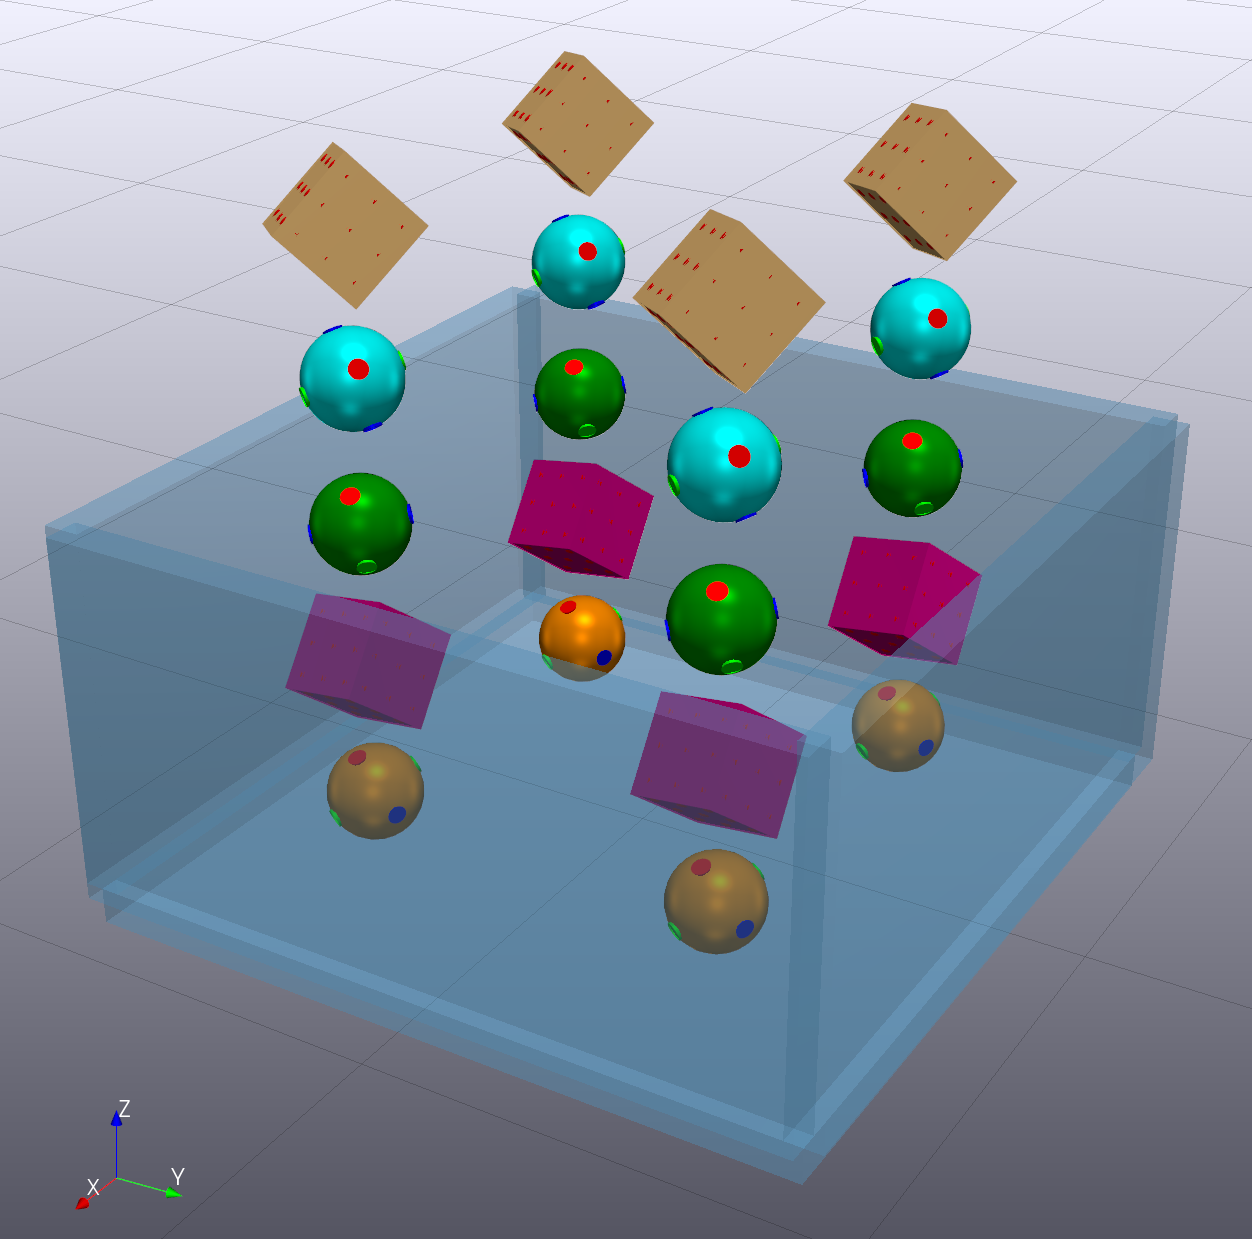
\includegraphics[height=0.44\columnwidth]{figures/pile_of_objects/clutter_t0.png}
	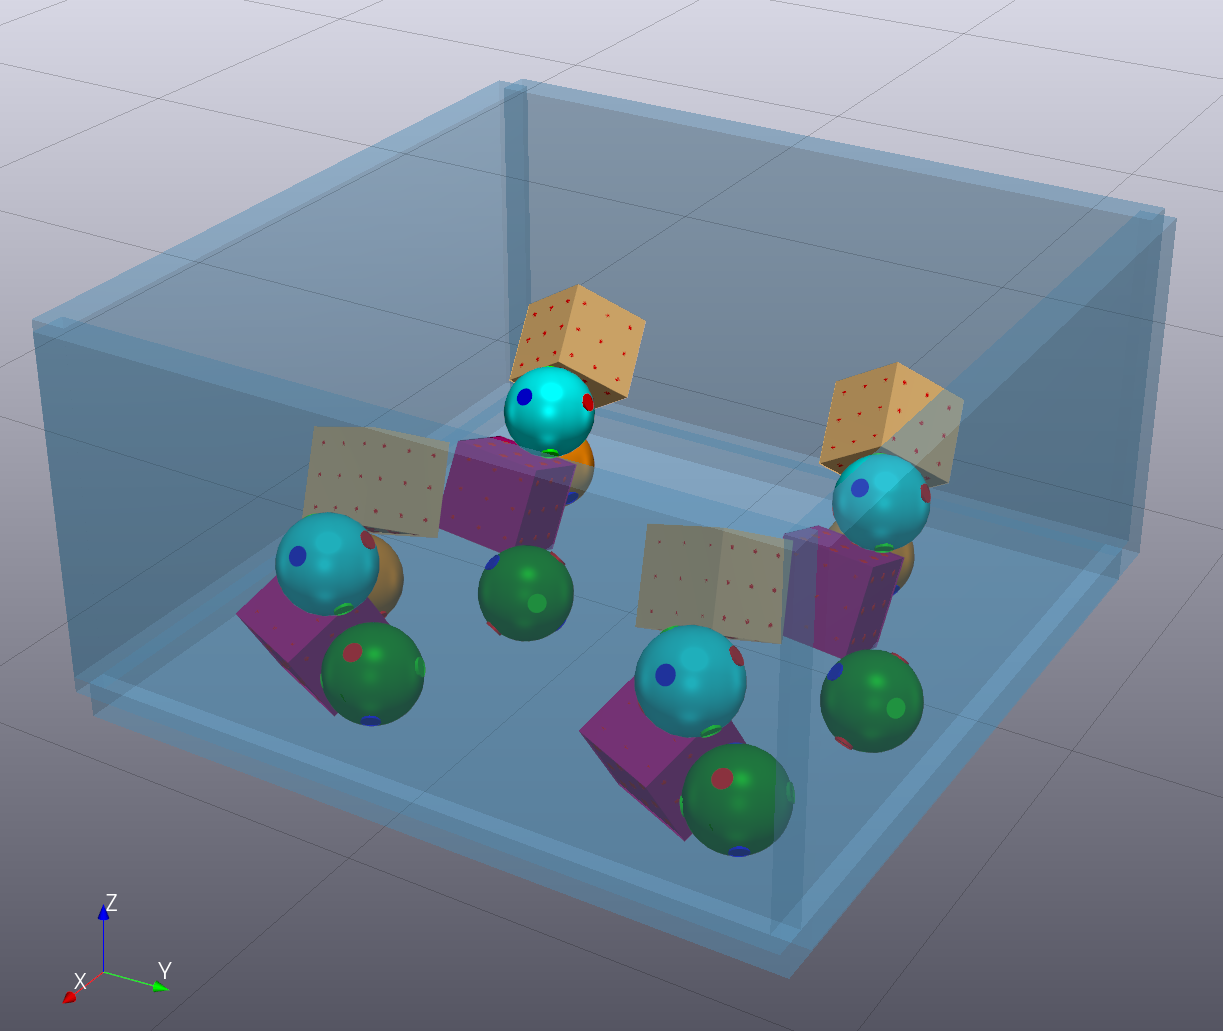
\includegraphics[height=0.44\columnwidth]{figures/pile_of_objects/clutter_t0p5.png}\\
	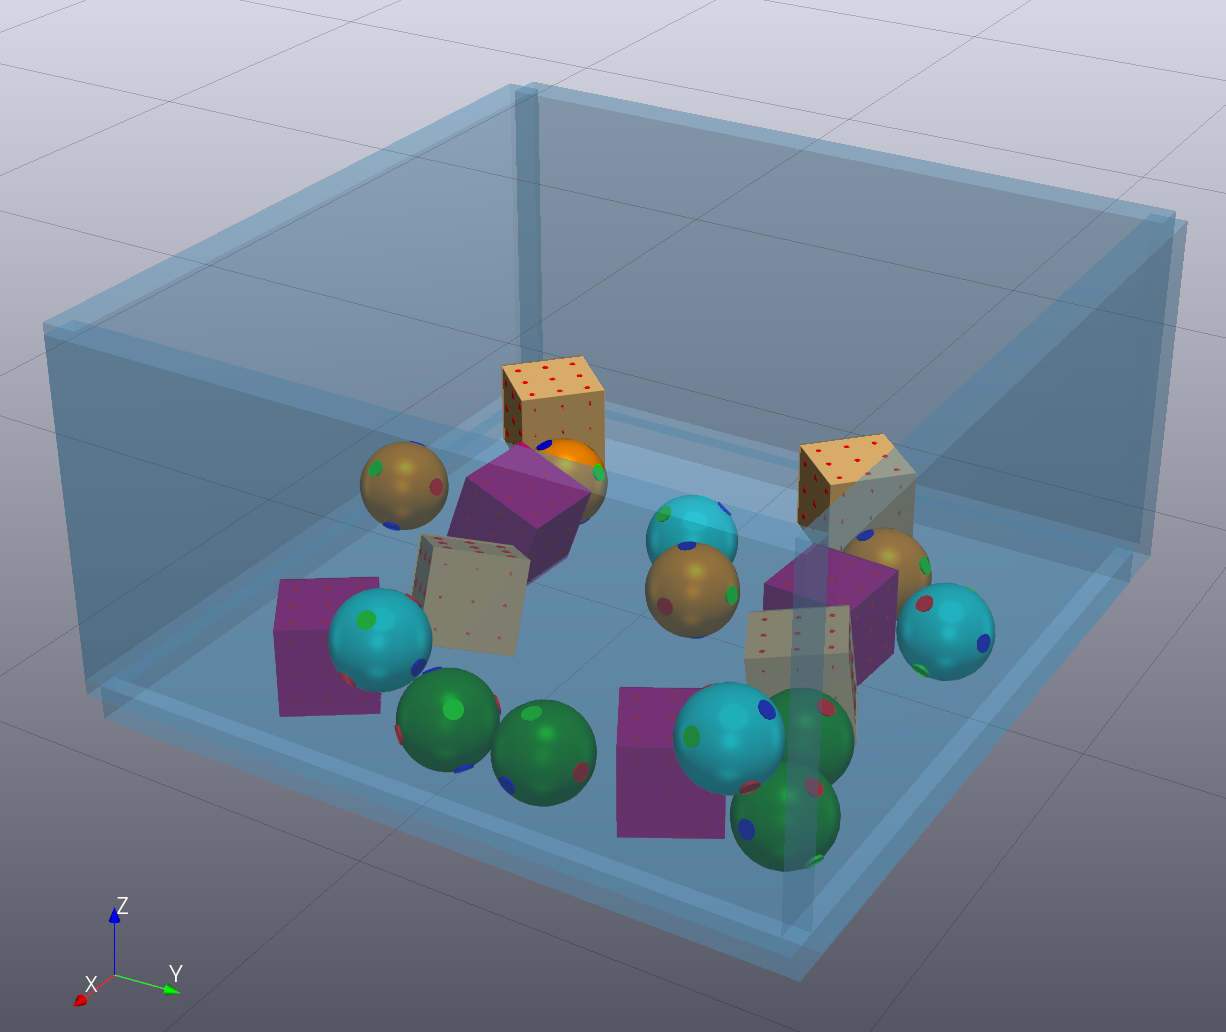
\includegraphics[height=0.4\columnwidth]{figures/pile_of_objects/clutter_t1p0.png}
	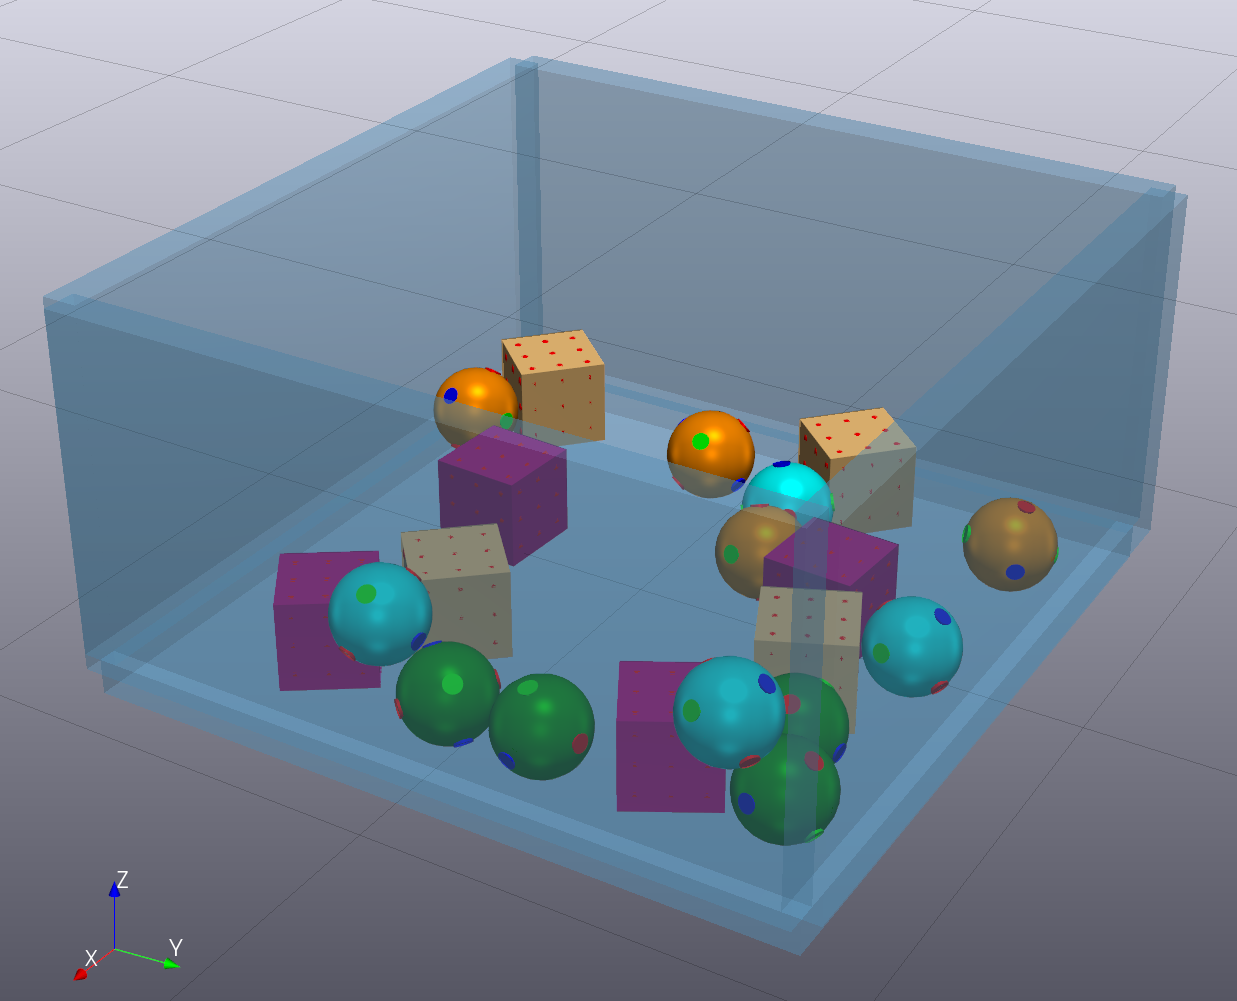
\includegraphics[height=0.4\columnwidth]{figures/pile_of_objects/clutter_t5p0.png}\\
	\caption{\label{fig:clutter} 
	Snapshots of the solution computed with time step $dt=10^{-2}~\text{s}$.
	From left to right, top to bottom, $t=0, 0.5, 1.0, 5.0\text{ s}$. }
\end{figure}

\begin{figure}[!h]
	\centering
	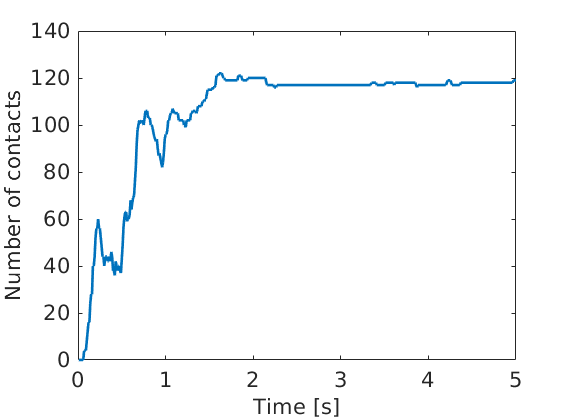
\includegraphics[width=0.45\columnwidth]{figures/pile_of_objects/number_of_contacts.png}
	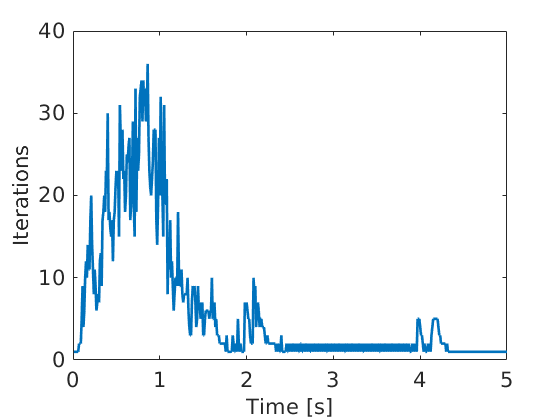
\includegraphics[width=0.45\columnwidth]{figures/pile_of_objects/newton_iterations.png}\\
	\caption{\label{fig:clutter_iterations} 
	Number of contacts and Newton iterations vs. time. }
\end{figure}

\begin{figure}[!h]
	\centering
	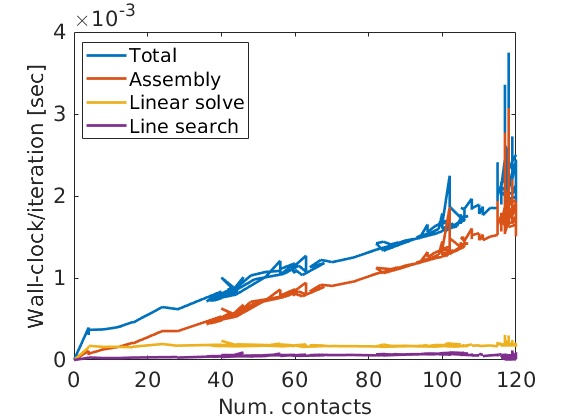
\includegraphics[width=0.45\columnwidth]{figures/pile_of_objects/wall_clock_vs_contacts.png}
	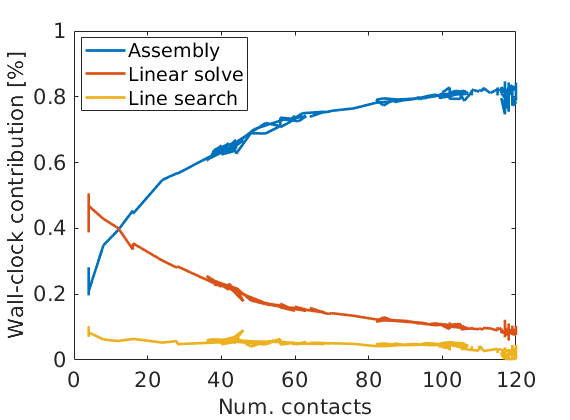
\includegraphics[width=0.45\columnwidth]{figures/pile_of_objects/wall_clock_contributions_vs_contacts.png}\\
	\caption{\label{fig:clutter_cost_budget} 
	Computational cost budget. Cost in seconds per Newton iteration (left) and
	percentile contribution per iteration (right).}
\end{figure}

